\documentclass[a4paper]{article}

\usepackage[utf8]{inputenc}
\usepackage[T1]{fontenc}
\usepackage{graphicx}
\usepackage[frenchb]{babel}
\usepackage{amsmath}
\usepackage{listings}
\usepackage{textcomp}
\usepackage{gensymb}

% define our color
\usepackage{xcolor}

% code color
\definecolor{ligthyellow}{RGB}{250,247,220}
\definecolor{darkblue}{RGB}{5,10,85}
\definecolor{ligthblue}{RGB}{1,147,128}
\definecolor{darkgreen}{RGB}{8,120,51}
\definecolor{darkred}{RGB}{160,0,0}

% other color
\definecolor{ivi}{RGB}{141,107,185}


\lstset{
    language=scilab,
    captionpos=b,
    extendedchars=true,
    frame=lines,
    numbers=left,
    numberstyle=\tiny,
    numbersep=5pt,
    keepspaces=true,
    breaklines=true,
    showspaces=false,
    showstringspaces=false,
    breakatwhitespace=false,
    stepnumber=1,
    showtabs=false,
    tabsize=3,
    basicstyle=\small\ttfamily,
    backgroundcolor=\color{ligthyellow},
    keywordstyle=\color{ligthblue},
    morekeywords={include, printf, uchar},
    identifierstyle=\color{darkblue},
    commentstyle=\color{darkgreen},
    stringstyle=\color{darkred},
}

\begin{document}

\title{VISA -- TP1 : Fuzzy Logic}
\author{Arnaud Cojez}
\date{mardi 18 octobre 2016}

\maketitle

\newpage
\tableofcontents
\newpage
%----------------------------------------------------------------------------------------
%	INTRODUCTION
%----------------------------------------------------------------------------------------

\section{Introduction}

\subsection{Motivation}
Dans le domaine de la reconnaissance de formes, la logique booléenne peut ne pas être suffisante. En effet, certains pixels sembleront appartenir à plusieurs zones d'une même image. Afin de définir à quelle zone appartient tel pixel, on utilise la logique floue.

\subsection{Explication}
Le principe de la logique floue est de non pas dire si un pixel appartient à une zone, mais de donner un pourcentage d'appartenance pour chaque zone.
Nous allons expliquer cette démarche le long de ce rapport.

\clearpage
%----------------------------------------------------------------------------------------
%	FONCTIONS D'APPARTENANCE
%----------------------------------------------------------------------------------------

\section{Fonctions d'appartenance}:

\subsection{Présentation du problème}

\subsubsection{Explication}
Nous sommes en présence d'une partition floue correspondant aux sous-ensembles flous suivants : Température Basse, Moyenne, Haute, associés à une variable Température (en °C) (Figure ci-dessous).

\begin{figure}[h]
\begin{center}
	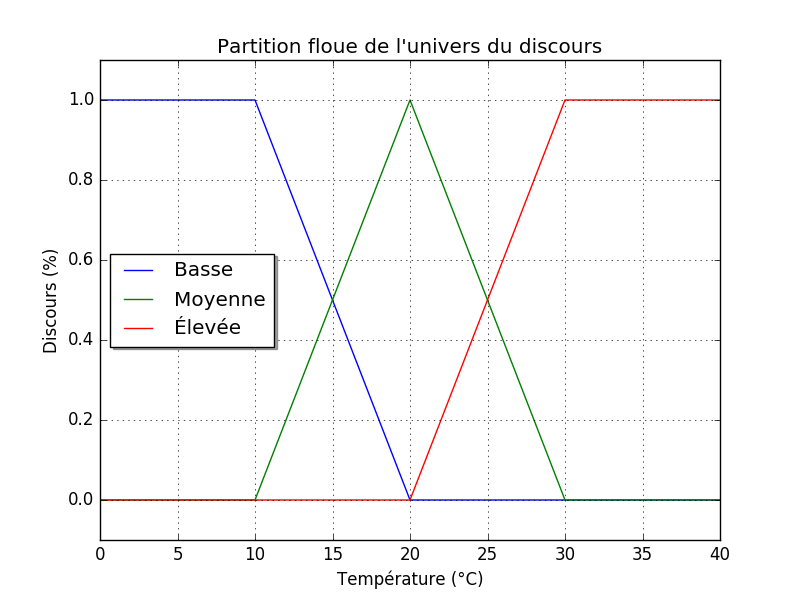
\includegraphics[width=400px]{plot_3.png}
\end{center}
\caption{Discours associé à la température en °C}
\end{figure}

Pour obtenir de telles courbes, il nous a fallu définir les fonctions ci-dessous.

\subsubsection{Implémentation Python}
\begin{lstlisting}
def basse(t):
    return np.clip((-t + 20.) * 0.1, 0., 1.)

def moyenne(t):
    return 1. - np.clip(np.sign(t - 20) * (t - 20) * 0.1, 0., 1.)

def elevee(t):
    return np.clip((t - 20.) * 0.1, 0., 1.)
\end{lstlisting}

Une fois ces fonctions définies, nous allons pouvoir dessiner les courbes ensemble sur un intervalle donné et obtenir le graphique montré plus haut.

\subsection{Degré d'appartenance}

\subsubsection{Explication}
Maintenant que nous avons les fonctions modélisant les différents discours, nous pouvons définir le discours associé à une température mesurée.
Ici nous prenons l'exemple de 16°C.

\begin{figure}[h]
\begin{center}
	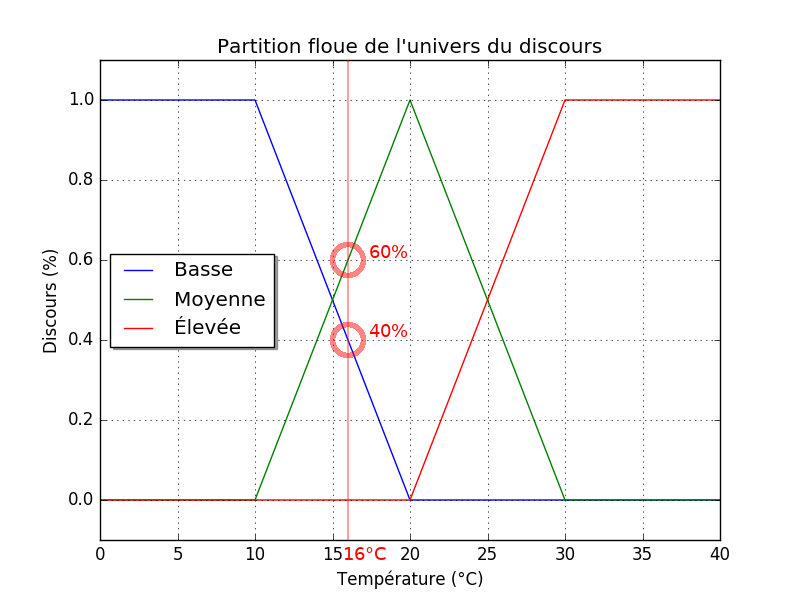
\includegraphics[width=400px]{plot_3_16dC.png}
\end{center}
\caption{Appartenance pour une température de 16°C}
\end{figure}

Nous voyons que la température de 16°C appartient à 40\% au discours "Température Basse" et à 60\% au discours "Température Moyenne", ce qui laisse apparaître une certaine transition dans le discours, transition qui n'est pas possible avec la logique booléenne.

Pour ce faire, nous avons besoin d'implémenter les fonctions et procédures suivantes :

\subsubsection{Implémentation}
\begin{lstlisting}
def get_appartenance(t):
    return [basse(t), moyenne(t), elevee(t)]

def print_appartenance(t):
    l = get_appartenance(t)
    print("Basse = ",l[0])
    print("Moyenne = ",l[1])
    print("Elevee = ",l[2])
\end{lstlisting}

\subsubsection{Trace}
Voici le résultat obtenu à l'éxecution :

\begin{lstlisting}[mathescape]
Question 2 : Appartenance de 16${^\circ}$C
Basse =  40.0 %
Moyenne =  60.0 %
Elevee =  0.0 %
\end{lstlisting}

\subsection{Température basse ou moyenne}

\subsubsection{Explication}
Nous pouvons utiliser des opérations logiques sur les ensembles de logique floue. Ci-dessous nous avons pour exemple l'ensemble flou "Température Basse OU Moyenne". Dans ce cas, l'opérateur OU peut-être remplacé par une fonction renvoyant le maximum (De même, ET sera remplacé par la fonction minimum).

\begin{figure}[h]
\begin{center}
	
\includegraphics[width=400px]{plot_basse_ou_moyenne.png}
\end{center}
\caption{Température basse OU moyenne}
\end{figure}

\subsubsection{Implémentation}

\begin{lstlisting}
  def basse_ou_moyenne(t):
  return np.maximum(basse(t), moyenne(t))
\end{lstlisting}


\clearpage
%----------------------------------------------------------------------------------------
%	Opérateurs de la logique floue
%----------------------------------------------------------------------------------------

\section{Opérateurs de la logique floue -BROUILLON}:

\subsection{Explication}

\subsection{Opérateur min}
\begin{lstlisting}
def op_min(fs, t):
    res = []
    for f in fs:
        if res == []:
            res = f(t)
        else :
            newRes = np.minimum(res, f(t))
            res = newRes
    return res
\end{lstlisting}

\begin{figure}[h]
\begin{center}
	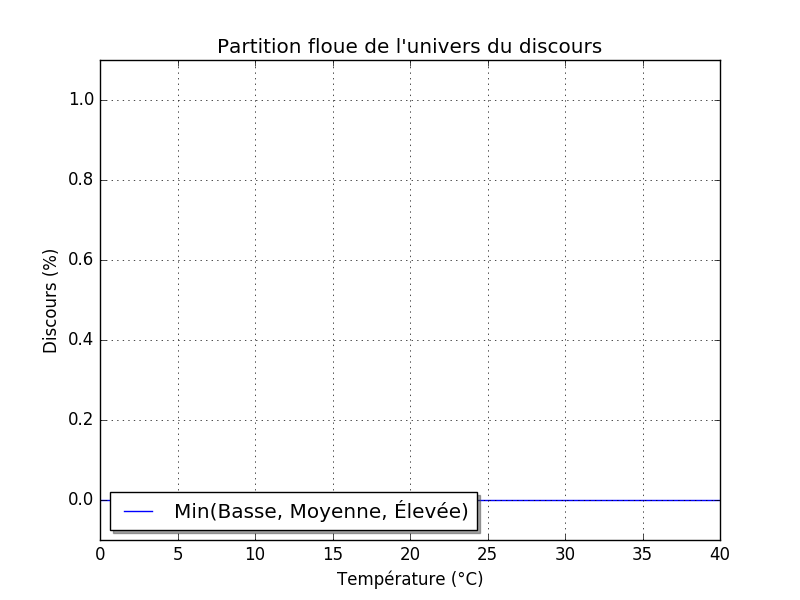
\includegraphics[width=400px]{plot_test_min.png}
\end{center}
\caption{min(Basse, Moyenne, Élevée)}
\end{figure}

\subsection{Opérateur max}
\begin{lstlisting}
def op_max(fs, t):
    res = []
    for f in fs:
        if res == []:
            res = f(t)
        else :
            newRes = np.maximum(res, f(t))
            res = newRes
    return res
\end{lstlisting}

\begin{figure}[h]
\begin{center}
	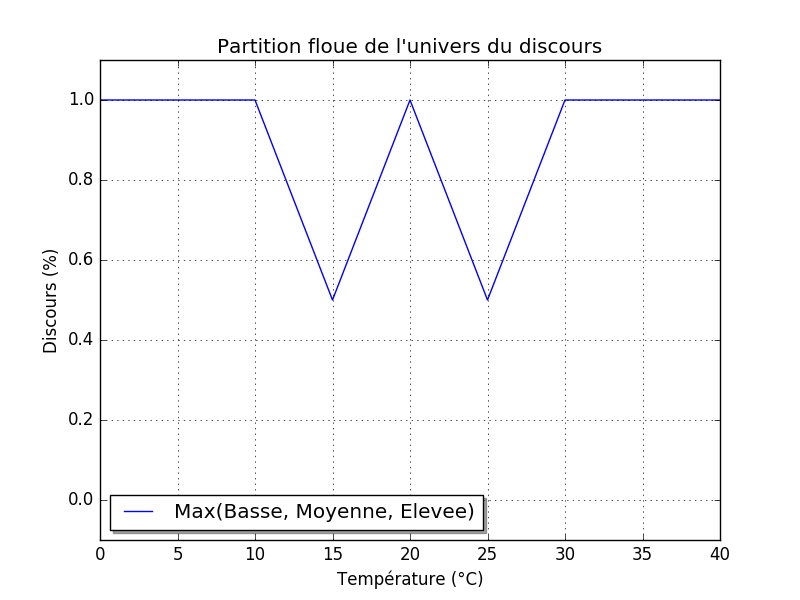
\includegraphics[width=400px]{plot_test_max.png}
\end{center}
\caption{max(Basse, Moyenne, Élevée)}
\end{figure}


\clearpage
%----------------------------------------------------------------------------------------
%	Implication floue
%----------------------------------------------------------------------------------------

\section{Implication floue -BROUILLON}:

\subsection{Règle floue R}
\begin{lstlisting}
def chauffer_fort(t):
    return np.clip((t - 8.) * 0.5, 0., 1.)
\end{lstlisting}

\begin{figure}[h]
\begin{center}
	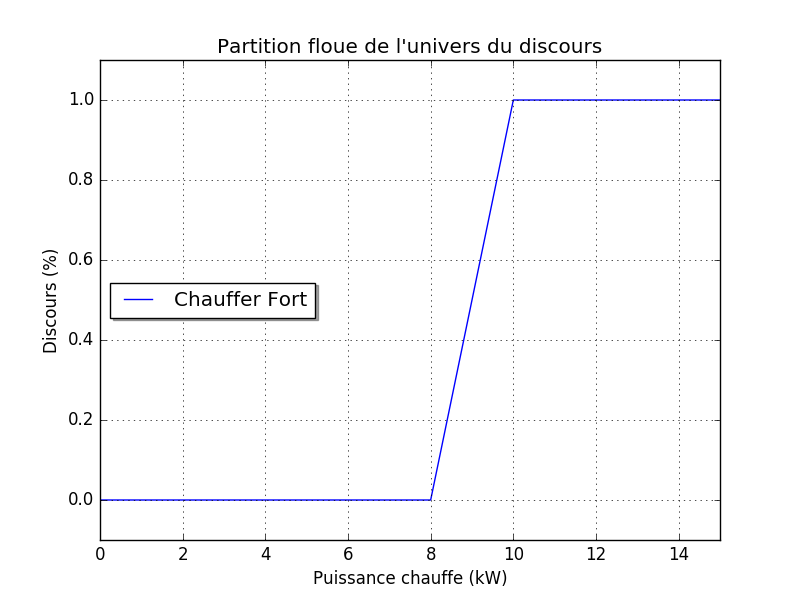
\includegraphics[width=400px]{chauffer_fort.png}
\end{center}
\caption{Discours Chauffer fort en fonction de la Puissance de Chauffe}
\end{figure}

\subsection{Implication de Mamdani}

\subsection{Ensemble flou de sortie}
\begin{lstlisting}
def mamdani(predicate, x0, conclusion, y):
    return np.minimum(predicate(x0), conclusion(y))))
\end{lstlisting}

\begin{figure}[h]
\begin{center}
	\includegraphics[width=400px]{{chauffer_fort_12.0}.png}
\end{center}
\caption{Implication de Mamdani Température/Chauffe pour 12°C}
\end{figure}


\clearpage
%----------------------------------------------------------------------------------------

%----------------------------------------------------------------------------------------
%	CONCLUSION
%----------------------------------------------------------------------------------------

\section{Conclusion -BROUILLON}

\end{document}
